\documentclass{school-22.211-notes}
\date{February 27, 2012}

\begin{document}
\maketitle

\lecture{Infinite Medium Resonance Cross Section Models}
\topic{NJOY Mechanism} % Lecture 6
Reference paper: `Methods for Processing ENDF/B-VII with NJOY' by R. E. MacFarlane and A.C. Kahler. \\
\uline{Basic idea}: we treat the resolved region and unresolved region separately: 
\begin{itemize}
\item Flux shape in resolved region: numerical solutions to the slowing down equations. For instance, if we consider an infinite homogeneous mixture of two materials and assume isotopic scattering in CMCS, then the integral slowing down equation is, 
\eqn{ \sigma(E) \phi(E) = \int_E^{E/\alpha_1} \frac{\sigma_{s1}(E')}{(1-\alpha_1)E'} \phi(E') \dE' + \int_E^{E/\alpha_2} \frac{\sigma_{s2} (E')}{(1-\alpha_2)E'} \phi(E') \dE' }
\item Flux shape in unresolved region: probability tables and analytic functions. Example: 
  \eqn{ \sigma_x(E) = \frac{\Sum_i \frac{P_i(E) \sigma_{xi}(E)}{\sigma_0 + \sigma_{ti}(E)} }{\Sum_i \frac{P_i(E)}{\sigma_0 + \sigma_{ti}(E)} } }
\end{itemize}
\uline{NJOY flow of codes}:
\begin{enumerate}
\item RECONR: reconstructs pointwise (energy-dependent) xs from ENDF resonance parameters (Reich-Moore) and interpolation schemes. 
\item BROADR: Doppler broadens and thins pointwise cross sections. There is no analytical way to Doppler broadening. 
\item UNRESR: unresolved range, we have probability table that tells you the distribution of resonance spacings etc. Analytical flux depression. 
\item HEATR: energy deficient. We do not really discuss this part. 
\item THERMR: deals with $S(\alpha, \beta)$ to treat chemical binding, etc that we skip.
\item GROUPR: important one. NJOY evaluates integral numerically, whereas We mimic this process using Monte Carlo because MC is easier to set up though is not as accurate. 
\item GAMINR: not that important. 
\end{enumerate}
We get multigroup cross sections out of NJOY. 
\begin{figure}[h]
  \centering
  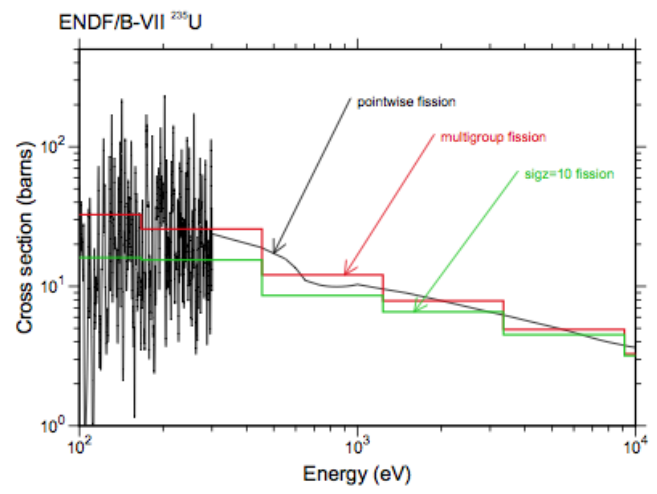
\includegraphics[width=0.45\linewidth]{images/r-m/mg-xs.png}
  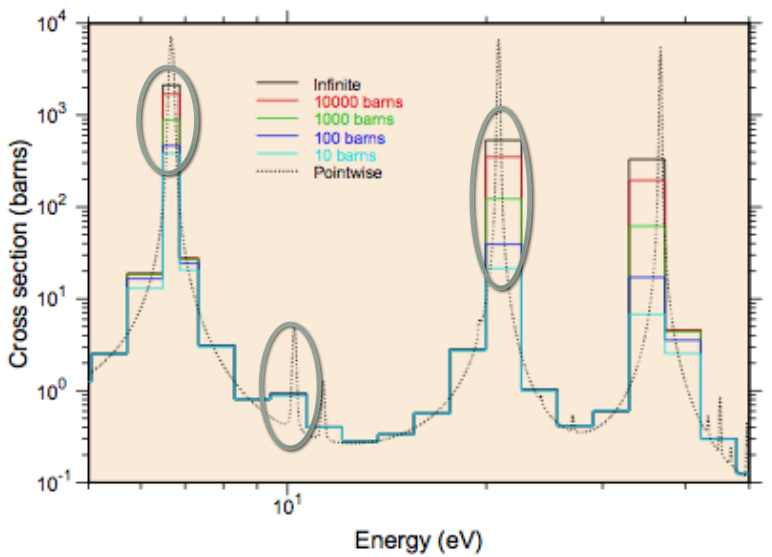
\includegraphics[width=0.45\linewidth]{images/r-m/mg-xs-2.png}
  \caption{Desired Product of NJOY: Multi-Group Cross Sections}\label{mg-xs}
\end{figure}
As illustrated in Fig.~\ref{mg-xs}, the multigroup cross section may differ by a factor of 10 depends on the resolution you run. Thus we cannot blindly use a set of multigroup cross sections without evaluating it specifically to a problem. Unless you are using 100,000 energy groups, \textit{no matter how good your spatial representation is, your results is no better than the multigroup cross sections you start out with.} 




\clearpage
\textbf{NJOY Flux Spectra Model and Resonance Model}
We assume a \textbf{homogeneous} system comprised of a moderator (m) and a resonance material (r) with a fission source. Then we can write the balance equation of consumption equals fission and scattering source: 
\eqn{ [N_R \sigma_t^R(E) + N_M \sigma_t^M(E)] \phi(E) &=
\chi(E) + \int_E^{E/\alpha_R} N_R \sigma_s^R(E'\to E) \phi(E') \dE' + \int_E^{E/\alpha_M} N_M \sigma_s^M(E'\to E) \phi(E') \dE'}
Further assume \textbf{scattering is isotropic in CMCS}, we write $\sigma_s(E' \to E) = \frac{\sigma_s(E')}{(1 - \alpha)E'}$: 
\eqn{ [N_R \sigma_t^R(E) + N_M \sigma_t^M(E)] \phi(E) &=
\chi(E) + \int_E^{E/\alpha_R} N_R \frac{\sigma_s^R(E')}{(1-\alpha_R)E'} \phi(E') \dE' + \int_E^{E/\alpha_M} N_M \frac{\sigma_s^M(E')}{(1-\alpha_M)E'} \phi(E') \dE'}
Assume the resonance region starts \textbf{well below the fission neutron emission energy region}, $\chi(E) \to 0$, and the \textbf{moderator scattering xs is independent of energy}, that is,$\sigma_s^M(E') \to \sigma_s^M, \phi(E') \to \frac{1}{E'}$,
\eqn{ [N_R \sigma_t^R(E) + N_M \sigma_t^M(E)] \phi(E) &=
\int_E^{E/\alpha_R} N_R \frac{\sigma_s^R(E')}{(1-\alpha_R)E'} \phi(E') \dE' + N_M \frac{\sigma_s^M}{1-\alpha_M} \int_E^{E/\alpha_M} \frac{1}{E'} \frac{1}{E'} \dE' \notag \\
 &=\int_E^{E/\alpha_R} N_R \frac{\sigma_s^R(E')}{(1-\alpha_R)E'} \phi(E') \dE' + N_M \frac{\sigma_s^M}{E} }
Assume the moderator has no absorption, on the LHS $\sigma_t^M(E) \to \sigma_s^M$, 
\eqn{ [N_R \sigma_t^R(E) + N_M \sigma_s^M] \phi(E) & =\int_E^{E/\alpha_R} N_R \frac{\sigma_s^R(E')}{(1-\alpha_R)E'} \phi(E') \dE' + N_M \frac{\sigma_s^M}{E} }
Recall the definition of background cross section $\displaystyle \sigma_b = \frac{N_R \sigma^M}{N_R}$, 
\eqn{ \Aboxed{[\sigma_t^R(E) + \sigma_b] \phi(E) & =\int_E^{E/\alpha_R} \frac{\sigma_s^R(E')}{(1-\alpha_R)E'} \phi(E') \dE' + \frac{\sigma_b}{E} } \label{resonance-model} }
Know this derivation in your sleep! 
\begin{itemize}
\item Only relative number density shows up in final equation.

\item More specifically, \hi{it is $\sigma_b$ that matters, not moderator species.} That is, $\sigma^M$ and number density ratio are imbedded in $\sigma_b$; if we pick a $\sigma_b$, and have a resonance absorber, then we can resolve the flux. If we switch the moderator species while keeping $\sigma_b$ constant, then the spectrum should be blind to the moderators. 

\item NJOY solves the above equation for any arbitrary cross sections of resonance material, so the flux shape can be arbitrarily complicated, including resonance scattering. 

\item Justification for assuming constant scattering cross section: main scatters are light isotopes, whose resonance energies are very high. Thus in the resonance range main scatters all have a constant scattering cross section. The only exception might be Na-23, as Na has a large scattering resonances at around 1 keV. Remember the heavier the isotope, the lower the resonance energies. 
\end{itemize}


\clearpage
\topic{Evaluating Monte Carlo Flux}
Eq.~\ref{resonance-model} provides the analytical resonance model. Alternatively, we can use Monte Carlo to tally flux by tallying $\displaystyle \frac{1}{\Sigma_t}$ at each collision, and tally RI (every time we say RI we mean absorption/capture, not scattering).  We tested for H/U = 100, A=1, 12, and 24: 
\begin{enumerate}
\item MC RI is pretty much independent of moderating/scattering material. In the analytical expression, $\phi(E)$ depends on . RI is not sensitive to moderating material mass because the resonance width is so narrow. 

\item MC RI has small sensitivity to the existance of resonance scatter. Adding in resonance scatter, RIs decrease slightly. 

\item A subtle point here is that the little increases in flux generated by resonance scatters. The reason is: 
 $\sigma_{po}^{238} = 13.9 \barn, \sigma_b = 100 \times 20 = 2,000 \barn$. \hi{At certain energies, resonance scattering xs exceeds resonance capture xs, adding a big extra slowing down source from scattering off U238.}
  \begin{figure}[h]
    \centering
    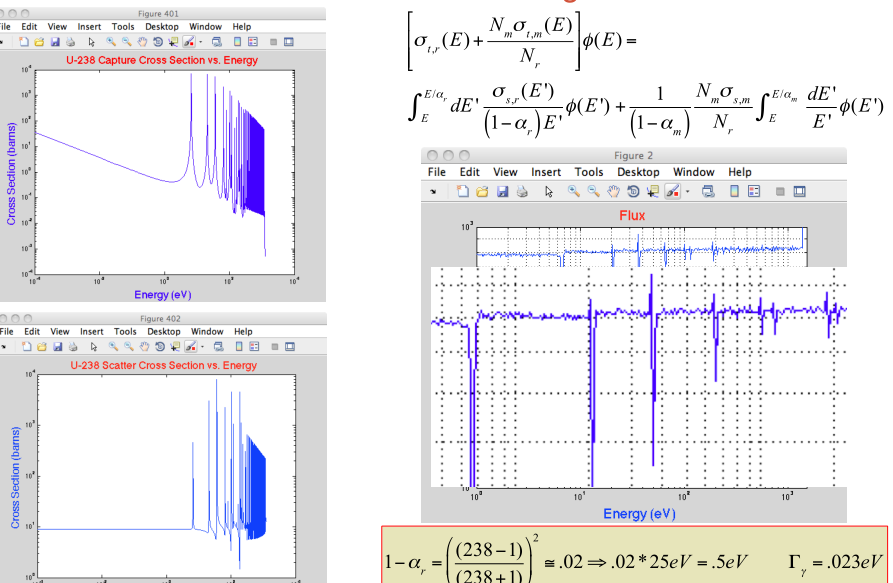
\includegraphics[width=4in]{images/r-m/res-scat.png}
    \caption{Resonance Scatters' Effects}
  \end{figure}
\end{enumerate}


 




\clearpage


\end{document}
